% sample.tex
\documentclass[graduation-thesis]{jsarticle}
	\usepackage[dvipdfmx]{graphicx}
	\usepackage{url}
	\usepackage{atbegshi}
	\AtBeginShipoutFirst{\special{pdf:tounicode EUC-UCS2}}
	\usepackage[dvipdfmx,setpagesize=false]{hyperref}
		\usepackage[dvipdfmx]{color}
\usepackage{url}
\usepackage{float}
\usepackage[setpagesize=false]{hyperref}
\usepackage{ascmac}
\usepackage{here}
\usepackage{txfonts}
\usepackage{listings, jlisting}
\author{61305507 情報工学科 勝又裕之}
\date{\today}
\title{}
\begin{document}


\makeatletter
\renewcommand{\thetable}{
	\thesection.\arabic{table}
} %「表(章番号)-#.」と表記するための措置
\@addtoreset{table}{section}

\renewcommand{\thefigure}{
	\thesection.\arabic{figure}
}
\@addtoreset{figure}{section} %「図(章番号)-#.」と表記するための措置

\setcounter{page}{1}

\pagenumbering{roman}
\tableofcontents
\clearpage

\pagenumbering{arabic}

\definecolor{keywords}{RGB}{255,0,90}
\definecolor{comments}{RGB}{0,0,113}
\definecolor{red}{RGB}{160,0,0}
\definecolor{green}{RGB}{0,150,0}
\lstset{
	basicstyle=\ttfamily\footnotesize,
	frame=single,
	keywordstyle=\color{keywords},
	commentstyle=\color{comments},
	stringstyle=\color{red},
	showstringspaces=false,
	identifierstyle=\color{green},
	}

\section{はじめに}
\label{intro}
 近年,マルチテナント型のクラウドにコンテナ技術が利用されている.マルチテナント型のクラウドの例として, Amazon Web Services や Google Cloud Platform がある.こういったクラウドを管理する場合に, isolation が重要である.ここで,isolation と throttle との違いを明確にしておく.ディスクへの書き込みを 15\% に制限しているが, 30\% 必要としているプロセスと, 85\% に制限しているが 50\% しか必要としていないプロセスを実行したとする.throttle であれば,前者はディスクへの書き込みを 15\% ,後者は 50\% の割合で使う.一方, isolation では,余っている分を自由に利用できるので,後者が 50\% しか利用していないため,前者は必要としている 30\% 分を使うことができる.\\
\begin{figure}[H]
	\begin{center}
		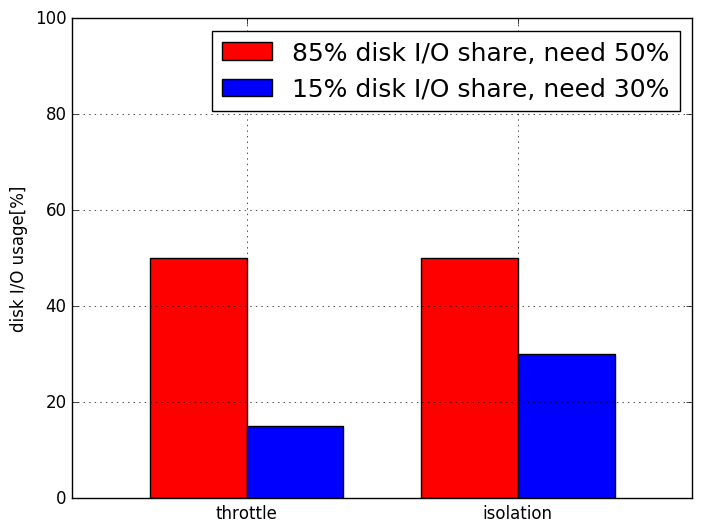
\includegraphics[width=7.5cm]{images/isolation.png}
		\caption{throttle と isolation との違い}
		\label{fig:isolation}
	\end{center}
\end{figure}
 コンテナ技術の一つとして, Linux コンテナ (LXC) がある.LXC は linux カーネル機能の一つである cgroup を利用して,コンテナ毎の資源管理を行っている.また,それによってコンテナ間の isolation を保っている.しかし, cgroup による isolation は不完全である.2個のコンテナを用意する.片方のコンテナでは cgroup によって disk I/O 使用率を 85\% に制限し,Flexible IO(FIO) write benchmark を実行する.もう一方のコンテナでは,disk I/O 使用率を 15\% に制限し,FIO write benchmark を 100 命令に一回 fsync しながら実行する.この状況では,disk I/O 使用率を 85\% に制限している方は,本来は 85\% 使えるはずが 40\% しか使えなかった.\\
 コンテナ環境における isolation の不完全性は, DDoS 攻撃への脆弱性となる可能性がある.本論文では,実際にコンテナ環境において利用される, MySQL と varmail に対して攻撃が可能であることを示し,その解析を行う.MySQL への攻撃が可能であるか検証するためコンテナを2つ用意する.片方のコンテナで, disk I/O 使用率を 85\% に制限して MySQL benchmark を実行する.もう一方のコンテナで, disk I/O 使用率を 15\% に制限して,ファイルのメタデータを頻繁に更新するスクリプトと FIO read benchmark を実行する. この時, MySQL は,本来 disk I/O を 85\% 使えるはずが,50\% しか使えていなかった.よって, MySQL に対して攻撃が可能だと言える.同様に, varmail への攻撃が可能であるか検証するためにコンテナを2つ用意する.片方のコンテナで disk I/O 使用率を 85\% に制限して varmail benchmark を実行する.もう一方のコンテナで, disk I/O 使用率を 15\% に制限して,ファイルのメタデータを頻繁に更新するスクリプトと FIO read benchmark を実行する.この時, varmail は,本来 disk I/O を 85\% 使えるはずが, 50\% しか使えていなかった.よって, varmail に対して攻撃が可能だと言える.\\
 cgroup による isolation が不完全な原因は,journal であった.LXC ではコンテナ間で file system を共有しているため,複数のコンテナの disk I/O が,一つの journal でシリアライズされる.攻撃側は,頻繁に fsync を呼び,メタデータを更新しようとしている.攻撃側の頻繁な更新リクエストにより, journal に負荷がかかる.これによって, disk I/O の遅延時間が増加するようになるが,一つの journal で管理していることによって,すべてのコンテナでこの影響を受ける.したがって,攻撃対象の遅延時間を増やし,パフォーマンスを下げることが出来たのだと考える.また,攻撃側の,メタデータの更新リクエストの頻度を上げるほど,攻撃対象の遅延時間は増加する傾向にあった.\\
 本論文の構成を以下に示す.
 第\ref{sec:LXC}章では,LXC の資源管理の仕組みについて説明する.
 第\ref{sec:journaling}章では,journaling file system の仕組みについて説明する.
 第\ref{sec:DDoS}章では,現在のコンテナ環境において, DDoS 攻撃が可能であることを示す.
 第\ref{analysis}章では, DDoS 攻撃が可能である原因を解析する.
 第\ref{relative}章では,本研究に関連する研究について紹介する.
 第\ref{conclusion}章では,まとめと今後の課題について述べる.
 
\clearpage
\section{Linux コンテナにおける資源管理}
\label{sec:LXC}
 近年,仮想化技術としてコンテナが注目されている.コンテナを実現する技術の一つに Linux コンテナ (LXC) がある.本章では, LXC の資源管理の仕組みについて説明をする.\\
 LXC は,一つのマシン上にコンテナという隔離空間を作り出す.コンテナは,プロセスを隔離空間に入れることによって作り出している.LXC は, Linux カーネル機能の一つである cgroup を使い,コンテナへの資源の割り当てを管理している.\\
 cgroup は, OS が管理する資源を一元的に管理できる Linux カーネル機能である.cgroup は,プロセス,ファイルシステム, CPU ,メモリ, block I/O デバイスなどの各種デバイスといった多種のものを管理できる. cgroup はサブシステムによって,これら資源を管理している.表\ref{tb:subsystem}に, cgroup のサブシステムとその機能を示す.\\
\begin{table}[htb]
	\begin{center}
		\caption{cgroup のサブシステムとその機能}
		\begin{tabular}{|c||l|} \hline
			サブシステム名 & 機能\\
			\hline \hline
			blkio & ブロックデバイスへの入出力アクセスの制限を設定する\\
			\hline
			cpu & CPU コアの時間配分の割合を設定する\\
			\hline
			cpuacct & タスクが消費する CPU 時間をレポートする\\
			\hline
			cpuset & 使用可能な CPU コア数を設定する\\
			\hline
			devices & デバイスへのアクセスを制御する\\
			\hline
			freezer & タスクの一時停止と再開を制御する\\
			\hline
			hugetlb & cgroup からの hugetlb の使用\\
			\hline
			memory & タスクによって使用されるメモリの制限を設定する\\
			\hline
			net\_cls & プロセスが発信するパケットに識別子を付与し,制御する\\
			\hline
			net\_prio & タスクのネットワークの優先度を動的に設定する\\
			\hline
			pids & 起動するプロセス数を制限する\\
			\hline
		\end{tabular}
		\label{tb:subsystem}
	\end{center}
\end{table}
\begin{figure}[H]
	\begin{center}
		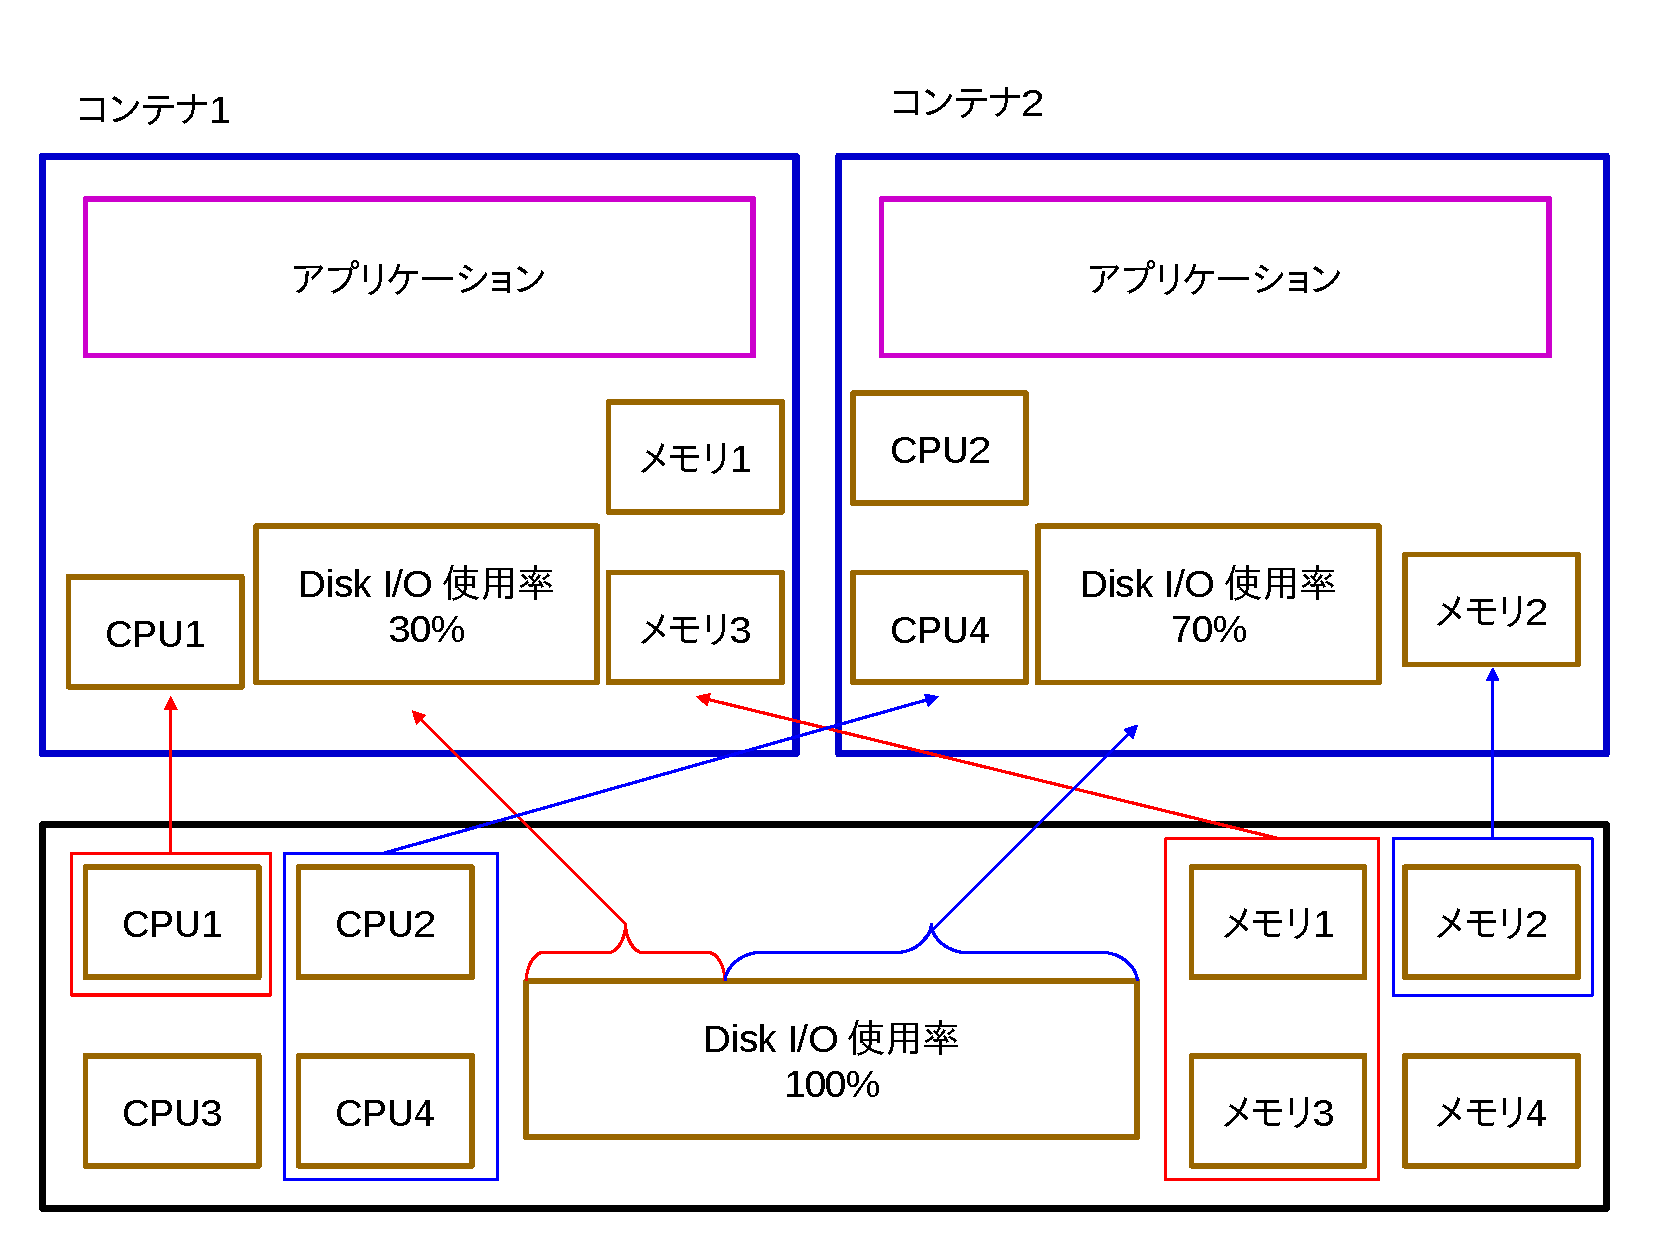
\includegraphics[width=10.0cm, clip]{images/container.pdf}
		\caption{LXC における資源管理の例}
		\label{fig:grouping}
	\end{center}
\end{figure}
 cgroup のグループを管理する方法は,おもに 5 つある.それは, cgroup ファイルシステムのマウント, cgroup の作成,プロセスの登録,プロセスの移動, cgroup の削除の 5 つである.
\begin{itemize}
	\item{cgroup ファイルシステムのマウント}\\
	cgroup は, /sys/fs/cgroup 以下にマウントされる.ここに,サブシステム名のディレクトリを作成する.すると,自動的に cgroup の使用状況を見たり, cgroup をコントロールしたりするためのファイルが作成される.例えば, /sys/fs/cgroup/cpu というディレクトリを作成すると, cpu ディレクトリ内に cpu.stat ファイルや cpu.shares ファイルなどが自動作成される.\\
	\item{cgroup の作成}\\
	cgroup を作成するには, cgroup のサブシステムのディレクトリ内に,適当な名前のディレクトリを作成する.例えば, /sys/fs/cgroup/cpu/test というディレクトリを作成すると, test という cgroup が作成でき, test ディレクトリ内に, cpu ディレクトリ内に作成されたファイルと同じ名前のファイルが自動作成される.\\
	\item{プロセスの登録}
	作成した cgroup にプロセスを登録する.作成した cgroup のディレクトリ内に自動作成されたファイルの一つに task ファイルがある.ここに,登録したいプロセスのプロセス ID を登録することで,プロセスを登録したことになる.また, cgroup に登録したプロセスの子プロセスや孫プロセスも自動的にその cgroup に登録される.例えば,現在起動しているシェルのプロセス ID が, 17899 であるとする.そこで, /sys/fs/cgroup/cpu/test/task に 17899 を書き込んで登録し, cat で task ファイルの中身を確認すると,シェルのプロセス ID 以外に,そのシェルで起動した cat のプロセス ID も表示される.\\
	\item{登録プロセスの移動}
	すでにある cgroup に登録してあるプロセスを,別の cgroup に登録する.これは,別の登録したい cgroup  側の task ファイルに,登録したいプロセスのプロセス ID を登録することで可能である.また,同時に二つの cgroup に,同じプロセスを登録することはできない.例えば, test1 と test2 という2つの cgroup があり, test1 の task ファイルには,プロセス ID が 17899 のプロセスが登録されているとする.このプロセスを test2 に登録するため, test2 の task ファイルに 17899 を登録する.その後, test1 の task ファイルの中身を確認すると, 17899 は消え, test1 には登録されていないことになっている.\\
	\item{cgroup の削除}
	cgroup を削除する方法は,通常のディレクトリを削除する方法と同様で, rmdir を使うことができる.ただし,その cgroup にプロセスが一つも登録されていないことが条件となる.\\
\end{itemize}
 以上のように cgroup は資源のグループ化を行い,グループごとに資源利用の優先度を決めたり,利用できる資源を制限したりしている.さらに,グループを隔離することで,他のグループから中が見えないようにしている.これによって,コンテナという隔離空間を作り出している.したがって,図\ref{fig:grouping}のように,あるコンテナから他のコンテナの内部へはアクセスが出来ない.\\
\begin{figure}[H]
	\begin{center}
		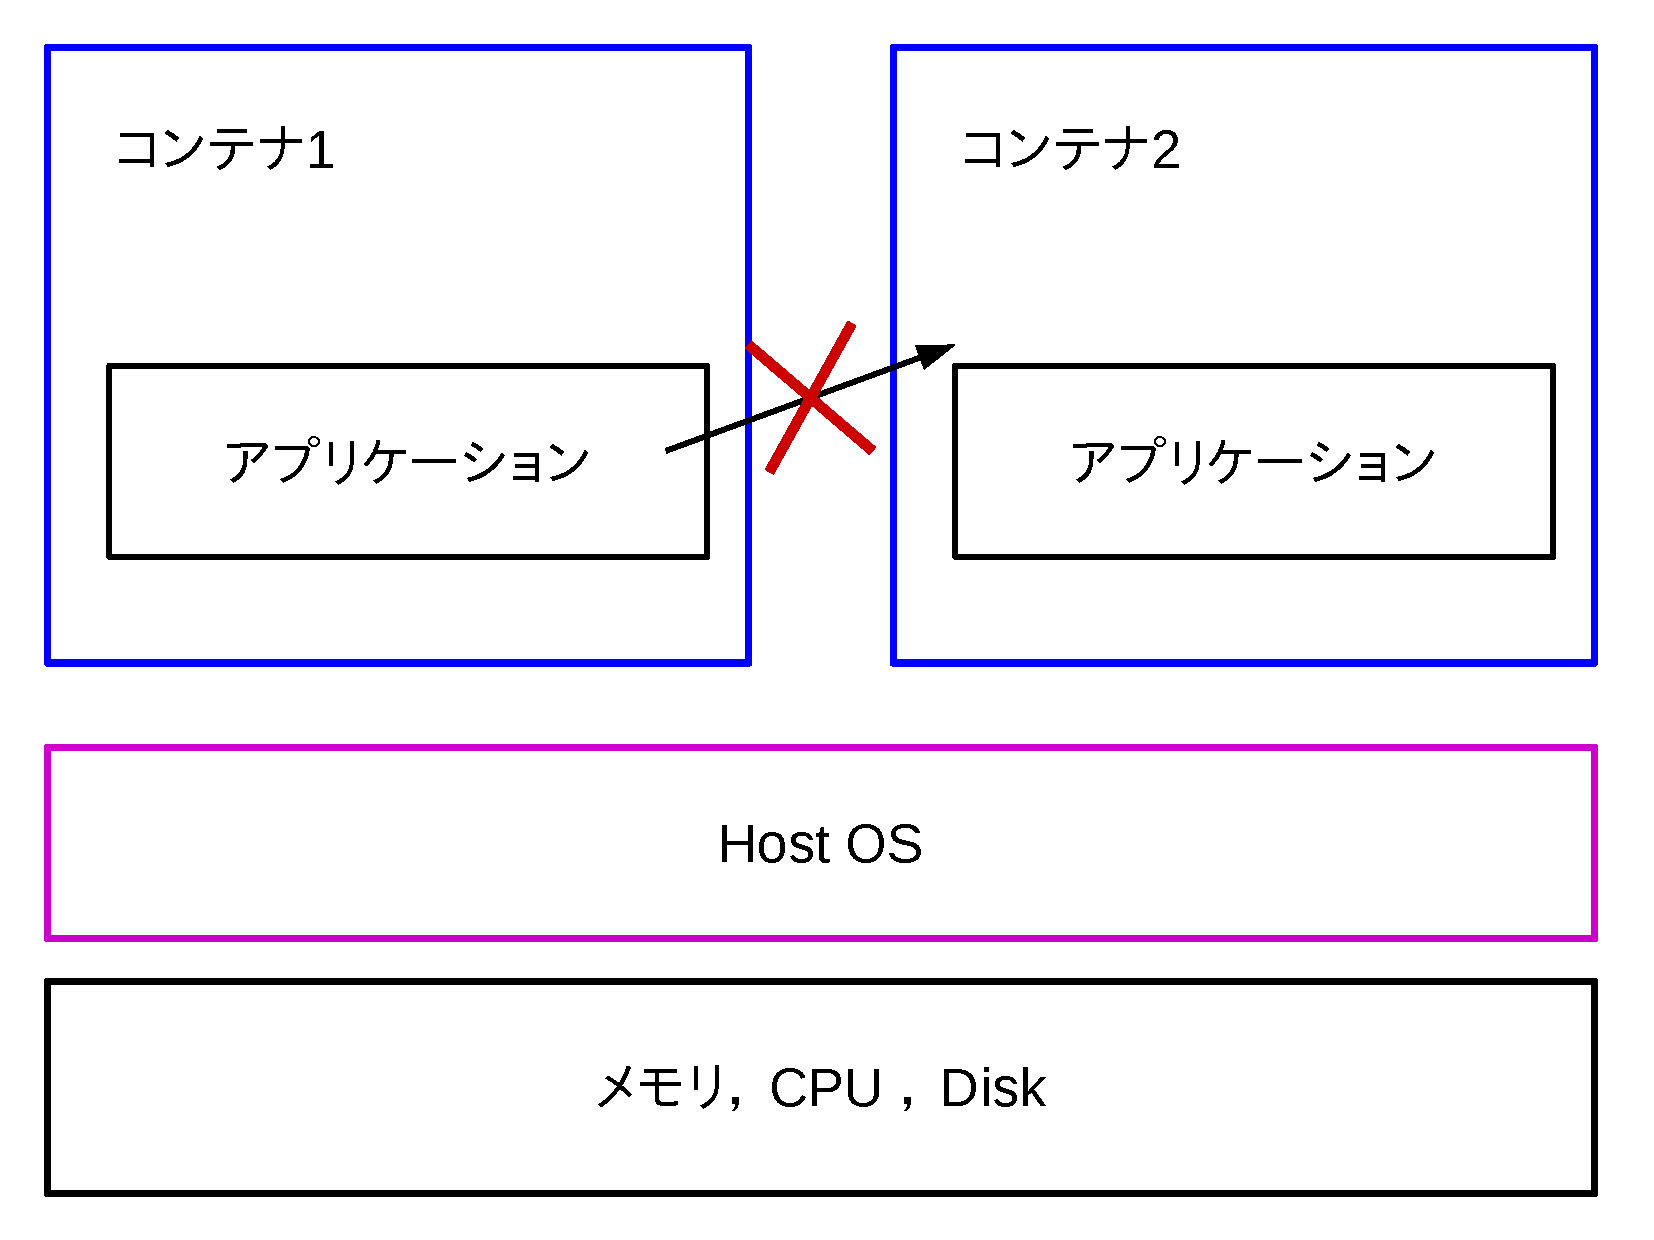
\includegraphics[width=5.0cm, clip]{images/kakuri.pdf}
		\caption{cgroup によるグループ化}
		\label{fig:grouping}
	\end{center}
\end{figure}
 より詳しく見ていくために, blkio サブシステムについて説明する。blkio サブシステムは, cgroup 内のタスクが行う,ブロックデバイス上の I/O アクセスを管理しする.制御の方法は,重み付け比例配分という方法と, I/O スロットリングという方法の2種類があります.I/O スロットリングは,特定のデバイスへの I/O 操作数の上限を設定するのに使います.重み付け比例配分は, Completely Fair Queuing スケジューラによりスケジューリングを行うことで,グループに重み付けをすることができる.この重み付けは, 100 ~ 1000 の間で指定できる.\\
 例えば,コンテナが2つある状況を考える.一方のコンテナのブロックデバイスへの I/O アクセスの重み付けを 850 に指定する.さらに,もう一方のコンテナの重み付けを 150 に指定する.これによって,片方のコンテナは,ブロックデバイスへの I/O アクセスを 85\% に制限され,もう一方は 15\% に制限されたことになる.ここで,両コンテナ上で Flexible I/O (FIO) benchmark を実行すると,図\{-----\}のようになる.また, FIO の設定は次のようになっている.workload の種類は sequential write である.キャッシュを使わないようにするため, Direct I/O で実行する.\\
 最後に, LXD について説明をする.LXD は LXC を操作するための REST API を提供するデーモンである.LXC は,コンテナの作成と管理を行うにあたって,十分な機能を持っているが,ユーザフレンドリではない.なぜなら, LXC のツールが何を行い,どのように動作するか,理解しておくべき知識が多くあるからだ.LXD では,こういった問題を解決し,動的なリソース制約やコンテナのマイグレーションなどの LXC では存在していた制約を解決することができると考えられている.
 
\clearpage
\section{journaling file system}
\label{sec:journaling}
 唐突な電源断が発生したり, OS にバグが発生したりすると, file system の一貫性が失われてしまう.この問題を crash-consistency problem という.本来,保存してあるデータは永続的なものであるべきである.そこで,この問題を解決するために生み出されたものが, journaling file system である.本章では, ext4 file system において,デフォルトで用いられている, metadata journaling について説明する.
\subsection{journaling の意味}
 本来,データは永続的なものであるべきである。しかし,データを変更する途中で,電源断が発生したり OS にバグが発生したりして,変更が中断されてしまう場合が存在する.この場合,復帰する際に特別な操作を行わないと, file system に矛盾が生じてしまう.簡単な書き込みを例に,途中でクラッシュが起こってしまった場合にどうなるかを紹介する.書き込み例は,すでに存在するファイルに対して,データブロックを一つ加えるもので,ファイルを開く,正しいオフセットの位置まで移動する, 4KB の write を発行する,ファイルを閉じるの 4 つの操作からなる.\\
 書き込み対象の file system も標準的な, inode bitmap, data bitmap, inodes, data blocks を含んでいるものとする.データ構造の初期状態を図\ref{fig:data1}に示す.inode bitmap Ba は,inode I[v1] が使用中であることを示している.data bitmap B[v1] は,data block Da が使用中であることを示している.inode I[v1] は,file size が 1 であり,ファイルの内容がブロック 4 ,つまり data block Da に格納されていることを示している.data block Da は,ファイルの内容を格納している.\\
\begin{figure}[H]
	\begin{center}
		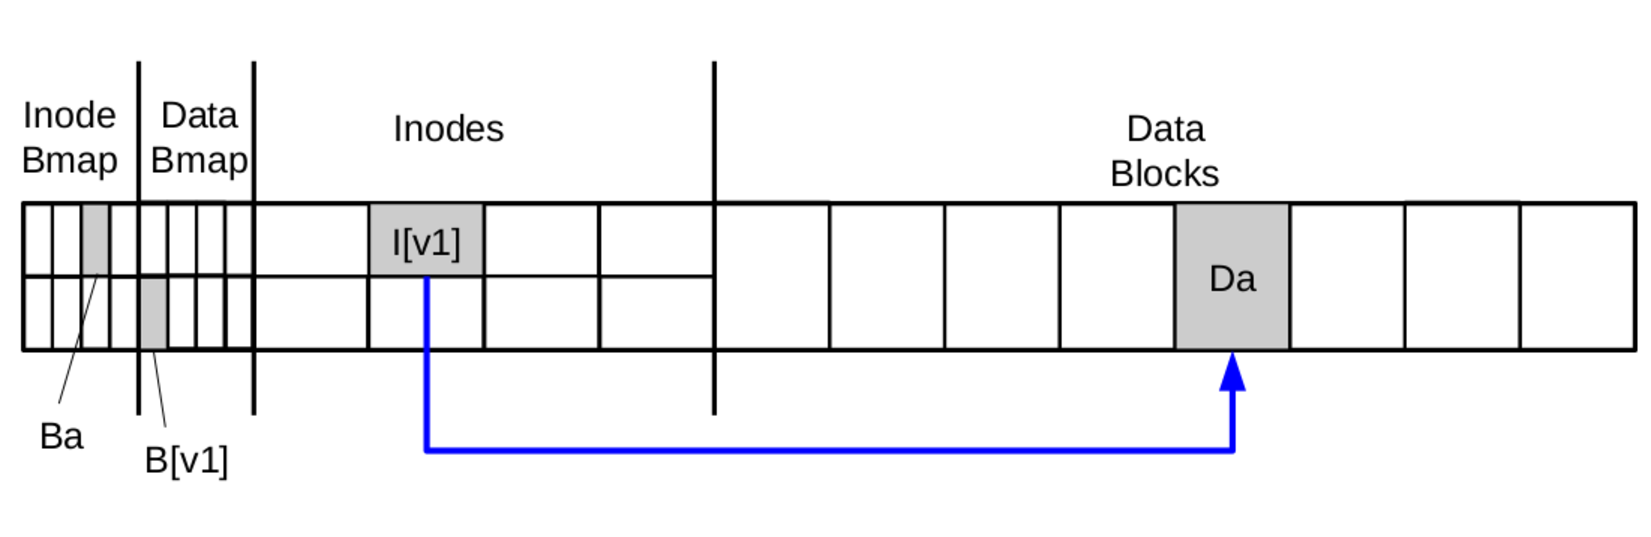
\includegraphics[width=15.0cm,clip]{images/data1.pdf}
		\caption{初期のデータ構造}
		\label{fig:data1}
	\end{center}
\end{figure}
 また, inode I[v1]の中身は表\ref{tab:inode1}のようになっているとする.\\
% この直後の表が来ないため,形を整える必要があるかもしれない.
\begin{table}[h]
	\begin{center}
	\caption{inode の初期状態}
		\begin{tabular}{lcl}
			owner & : & hoge \\
			permissions & : & read-write \\
			size & : & 1 \\
			pointer & : & 4 \\
			pointer & : & null \\
			pointer & : & null \\
			pointer & : & null
		\end{tabular}
		\label{tab:inode1}
	\end{center}
\end{table}
 1 ブロック分が割り当てられているので file size は 1, pointer はブロック 4 を指している.ここに,簡単な書き込み操作を行うと, data bitmap, inode, data block の 3 箇所が更新される.data block では,新しく data block Db が,ファイルに割り当てられる.inode I[v1] の pointer が,元々割り当てられている data block Da 以外に,新しく割り当てられた data block Db も指すようになり,file size は 2 となる.さらに, 新しく data bitmap B[v2] が, data block Db が使用されていることを指し示すようにする.無事,書き込み操作が行われた場合, inode I[v1] は表\ref{tab:inode2}のようなる.\\
\begin{table}[h]
	\begin{center}
	\caption{inode の書き込み操作終了後の状態}
		\begin{tabular}{lcl}
			owner & : & hoge \\
			permissions & : & read-write \\
			size & : & 2 \\
			pointer & : & 4 \\
			pointer & : & 5 \\
			pointer & : & null \\
			pointer & : & null
		\end{tabular}
		\label{tab:inode2}
	\end{center}
\end{table}
 さらに,書き込み操作終了後のデータ構造は図\ref{fig:data2}のようになる.\\
\begin{figure}[H]
	\begin{center}
		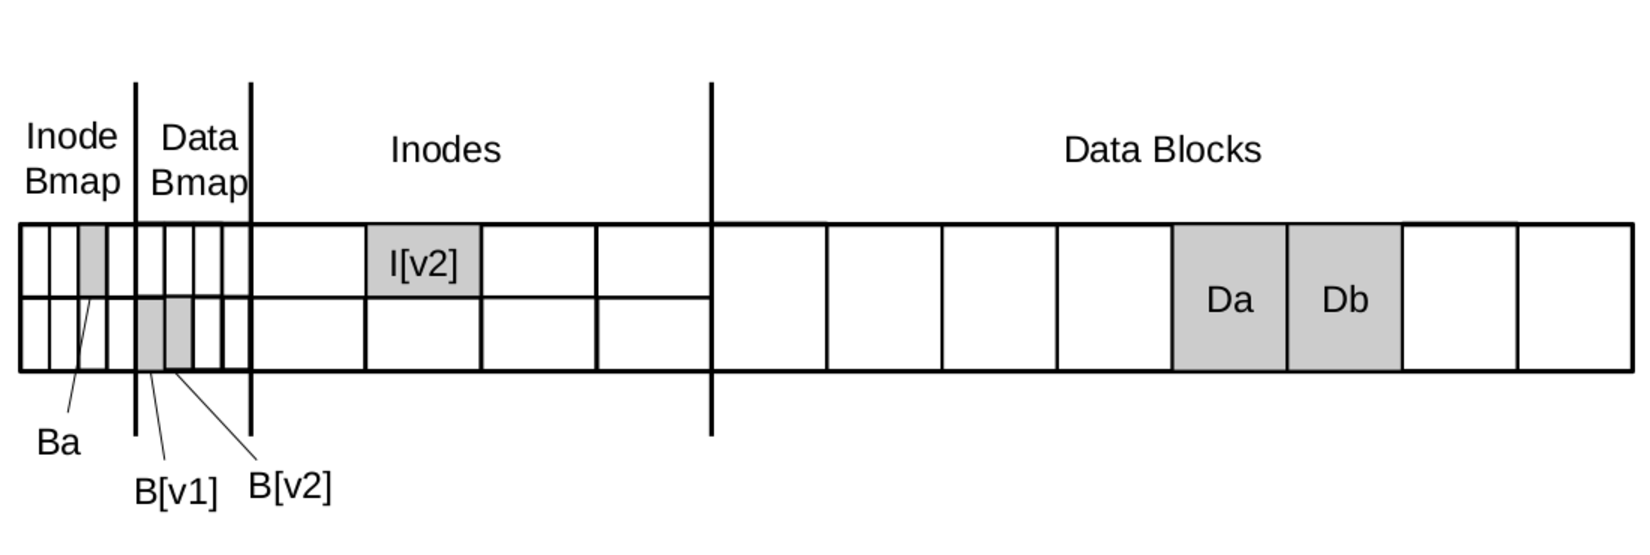
\includegraphics[width=15.0cm,clip]{images/data2.pdf}
		\caption{書き込み終了後のデータ構造}
		\label{fig:data2}
	\end{center}
\end{figure}
 上記で述べたとおり,書き込みの際に更新するのは,data bitmap, inode, data block の 3 箇所である.3 箇所の内, 1 箇所のみ,または 2 箇所の更新が終わった時点で,障害が発生した場合を説明する.
\begin{itemize}
	\item{data block Db のみ書き込みが完了した場合}\mbox{}\\
 この場合,データは disk に書き込まれているが, inode はそのブロックを指し示していない.さらに, data bitmap を見ても,そのブロックが使用されていないと表示されている.これは,書き込み操作が行われなかった場合とほぼ同じであるため,問題がないと言える.\\
\begin{figure}[H]
	\begin{center}
		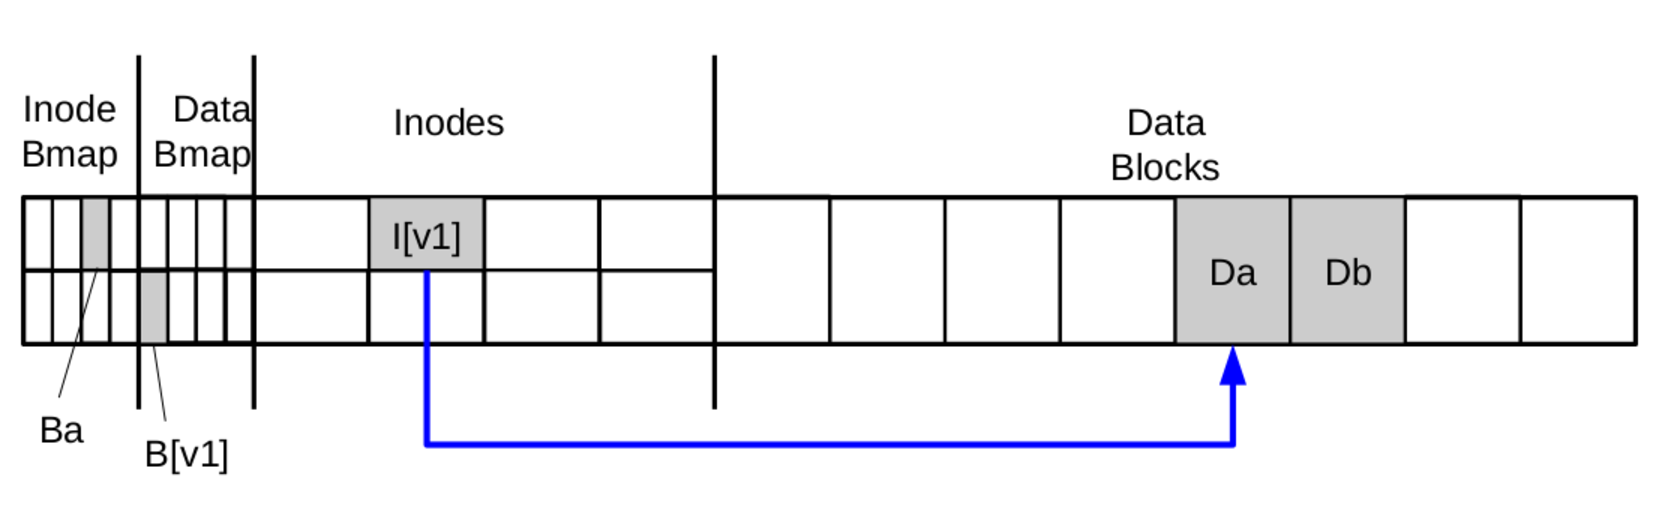
\includegraphics[width=15.0cm,clip]{images/data3.pdf}
		\caption{data block Db のみ書き込んだ場合}
		\label{fig:data3}
	\end{center}
\end{figure}
	\item{inode I[v2] のみ書き込みが完了した場合}\\
 この場合,data block Db の中身が書き込まれていないにもかかわらず, inode I[v2] の pointer は data block Db を指している状態になる.そのため, garbage data を読んでしまう可能性が存在する.さらに, inode I[v2] の pointer は data block Db を指しているが, data bitmap は,data block Db が使われていない状態であることを示している.つまり, file system の一貫性が崩れた状態となり,問題があると言える.\\
\begin{figure}[H]
	\begin{center}
		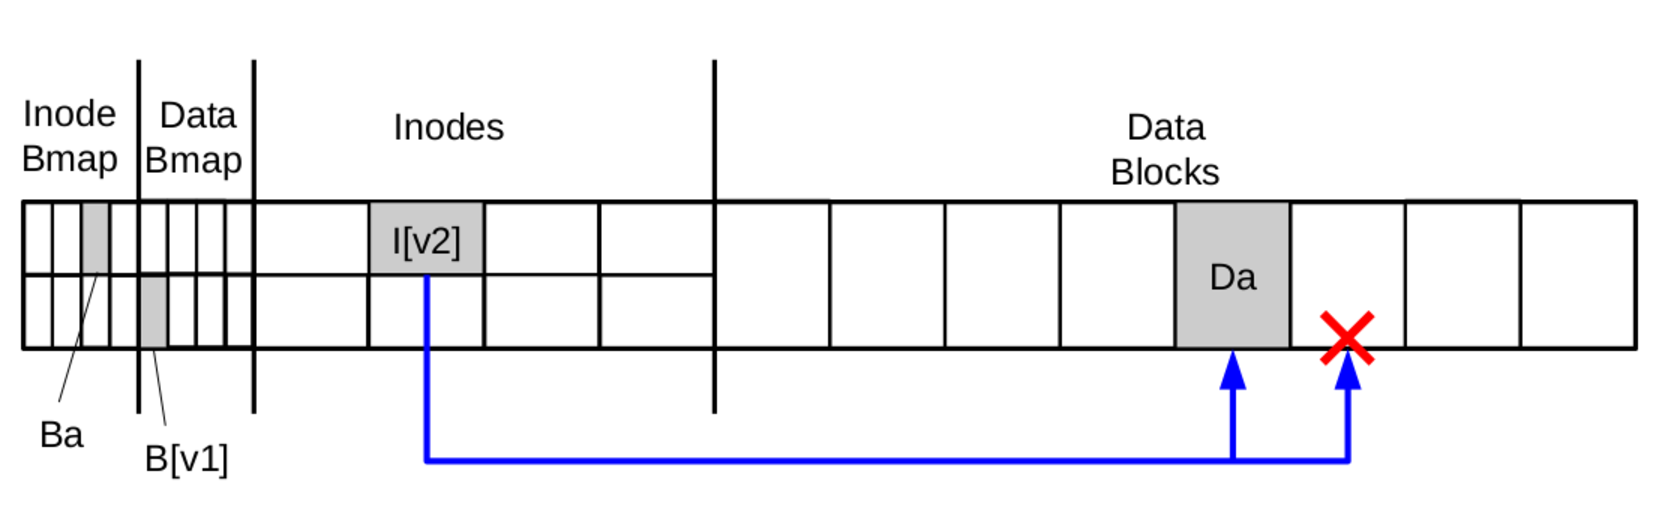
\includegraphics[width=15.0cm,clip]{images/data4.pdf}
		\caption{inode I[v2] のみ書き込んだ場合}
		\label{fig:data4}
	\end{center}
\end{figure}
	\item{data bitmap B[v2] のみ書き込みが完了した場合}\\
 この場合, data bitmap B[v2] は, data block Db が使用中であると示しているが,どの inode も data block Db を指していない.したがって,この場合も file system の一貫性が崩れた状態となり,さらに,data block Db が全く使えない状態に陥ってしまう.よって,問題があると言える.\\
\begin{figure}[H]
	\begin{center}
		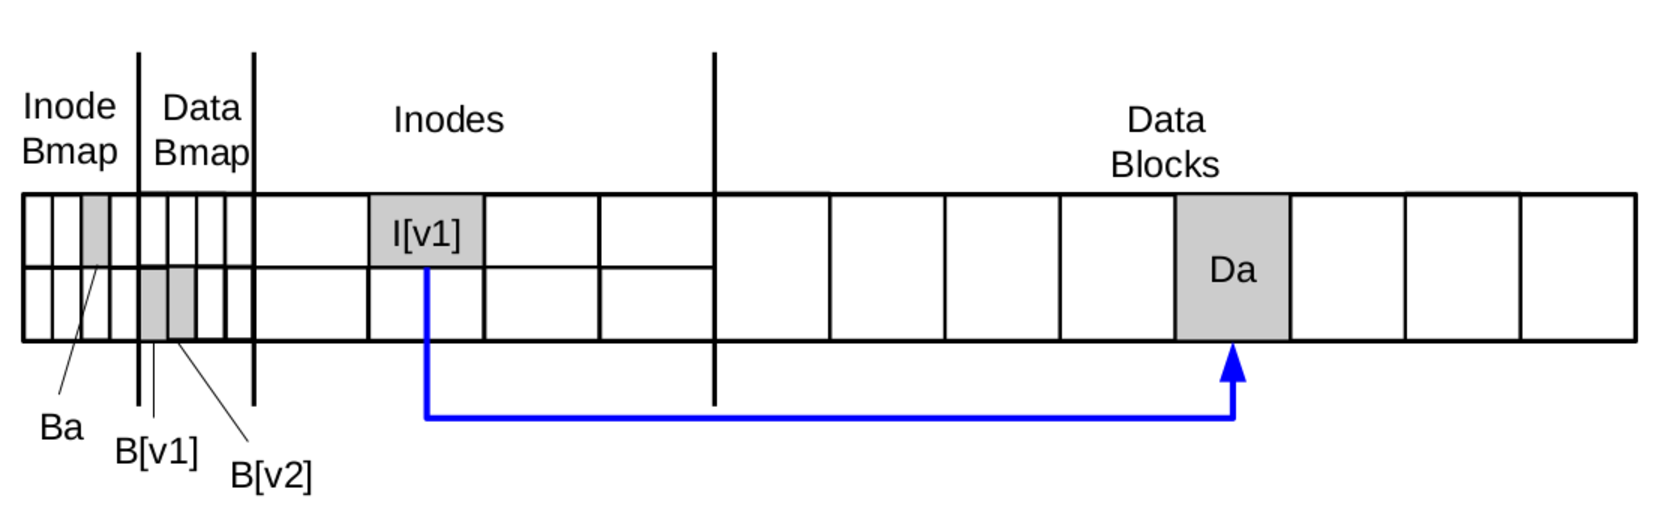
\includegraphics[width=15.0cm,clip]{images/data5.pdf}
		\caption{data bitmap B[v2] のみ書き込んだ場合}
		\label{fig:data5}
	\end{center}
\end{figure}
	\item{inode I[v2] と data bitmap B[v2] のみ書き込みが完了した場合}\\
 この場合, data bitmap B[v2] は, data block Db が使用中であることを示し, inode I[v2] はそのブロックを指している.よって,メタデータの一貫性は保たれている.しかし, data block Db の中身は書き込まれていないため, garbage data を読んでしまう可能性がある.したがって,問題があると言える.\\
\begin{figure}[H]
	\begin{center}
		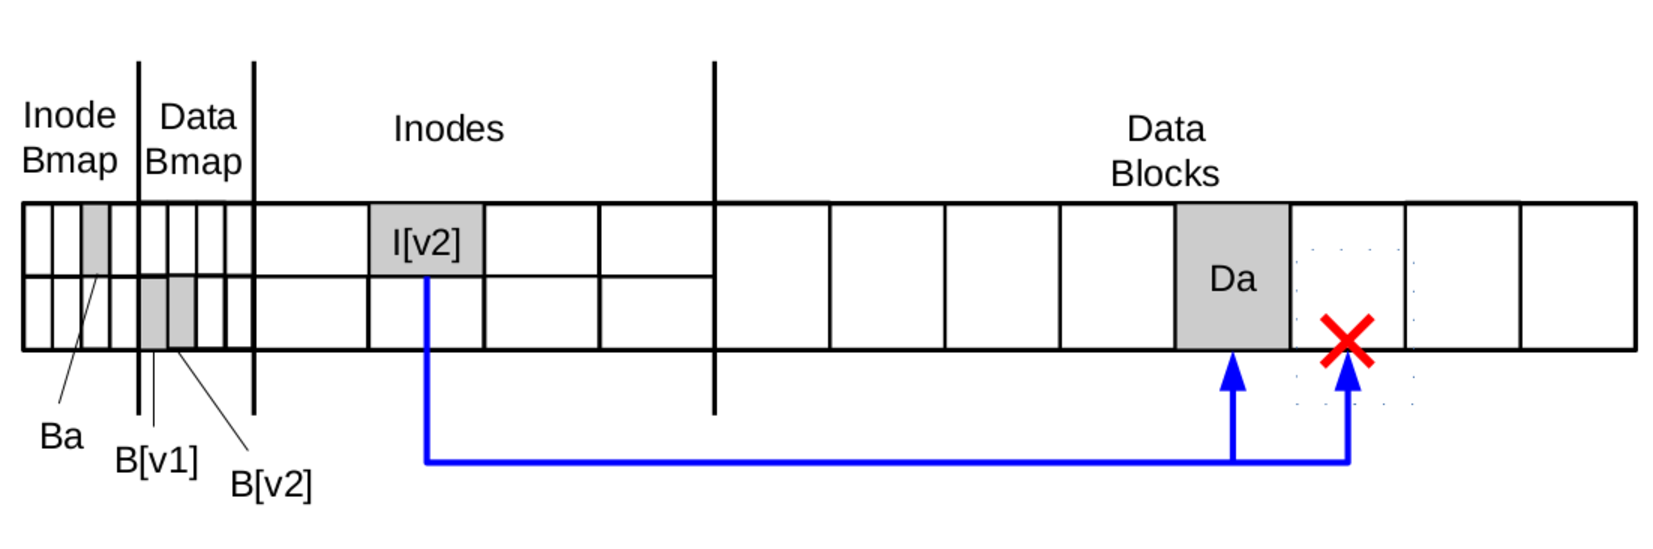
\includegraphics[width=15.0cm,clip]{images/data6.pdf}
		\caption{inode I[v2] と data bitmap B[v2] のみ書き込んだ場合}
		\label{fig:data6}
	\end{center}
\end{figure}
	\item{inode I[v2] と data block Db のみ書き込みが完了した場合}\\
 この場合, inode I[v2] の pointer は data block Db を指しており,中身も書き込まれているが, data bitmap B[v2] は data block Db が使用されていないと示している.これは, file system の一貫性が崩れた状態であり,問題があると言える.\\ 
\begin{figure}[H]
	\begin{center}
		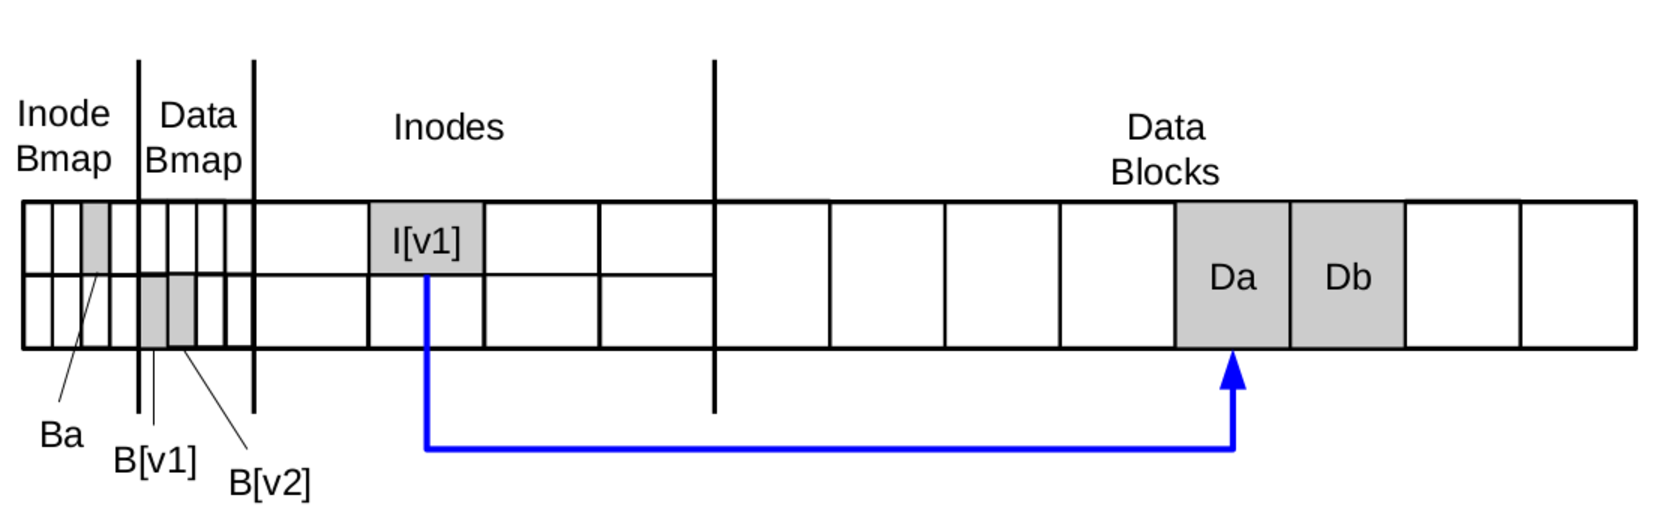
\includegraphics[width=15.0cm,clip]{images/data7.pdf}
		\caption{inode I[v2] と data block Db のみ書き込んだ場合}
		\label{fig:data7}
	\end{center}
\end{figure}
	\item{data bitmap B[v2] と data block Db のみ書き込みが完了した場合}\\
 この場合でも, inode I[v2] と data bitmap B[v2] との間に矛盾が生じているため, file system の一貫性が崩れている.	data block Db は使用されている状態にあり,中身も書き込まれているが,どのファイルに属すブロックかわからない.したがって,問題があると言える.\\
\begin{figure}[H]
	\begin{center}
		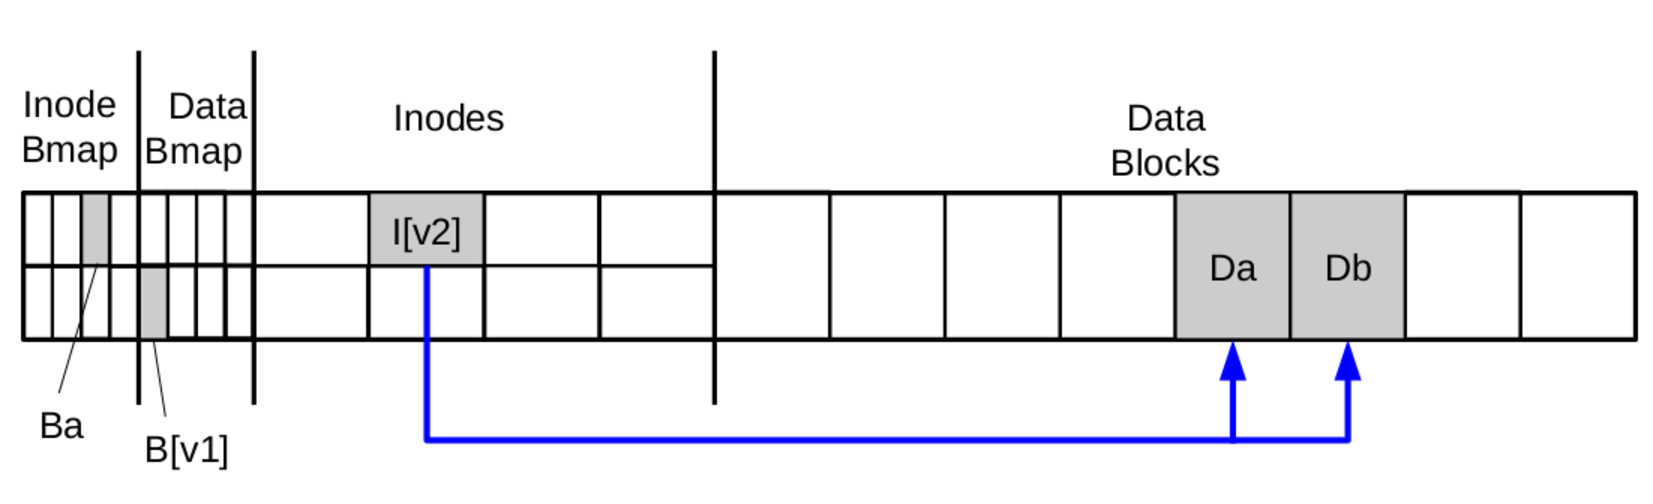
\includegraphics[width=15.0cm,clip]{images/data8.pdf}
		\caption{data bitmap B[v2] と data block Db のみ書き込んだ場合}
		\label{fig:data8}
	\end{center}
\end{figure}
\end{itemize}
 これらのクラッシュが起こった状況から見られるように,一部のブロックが使えなくなる状況が発生したり, garbage data をユーザに返してしまう状況が発生したりする.クラッシュが発生し,復帰したあとでも, file system に一貫性が保たれている状態にしたい.一方で, disk に対して一度に一つの write しか commit できないという制限がある.その制限の中で,クラッシュ後も file system が一貫性を保った状態で復帰できるようにするため, file system checker が生まれ,その後にそれを改良した journaling が生まれた.\\
\subsection{journaling の手順}
% まず,先に生まれた file system checker がどういった処理を行うか説明する.その後, journaling がどういった処理をするか説明する.\\
 journaling は, write ahead logging とも呼ばれる.disk の内容を更新する時に,これから実行しようとしていることをメモとして書いておく.これが ``write ahead'' の部分である.このようにすることで,データ構造の更新中にクラッシュが起きても,復帰時にメモしてあるものを見て,どういった操作をすればいいかわかるとともに,操作をやり直すことができる.また,クラッシュから復帰した際に,file system の一貫性が崩れていないか,ファイルを一つ一つ調べる必要がない.結果として,クラッシュ後の復帰時にメモを見るという少しの作業しかしなくても済むのである.\\
 journaling を使っていない ext2 file system と journaling を使っている ext3 file system を比較する.ext2 file system を見てみる.disk は一つの superblock と複数の block group に分けられている.さらに, block group は, inode bitmap, data bitmap, inode, data block からなる.superblock は file system の管理情報を記録する領域である.ext2 file system の構造は,図\ref{fig:ext2}のようである.\\
\begin{figure}[H]
	\begin{center}
		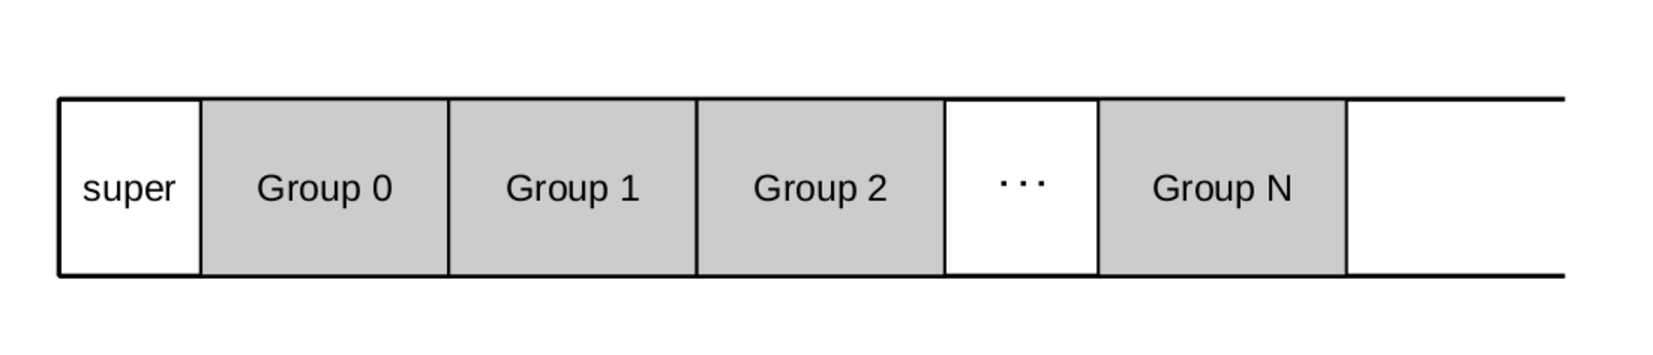
\includegraphics[width=15.0cm,clip]{images/ext2.pdf}
		\caption{ext2 file system の構造}
		\label{fig:ext2}
	\end{center}
\end{figure}
 ext3 file system は, ext2 file system に journaling 機能を足したものである.journaling 機能を満たすため,先ほど述べたメモを取るような領域を確保しておかなければならない.ext3 file system の構造は,図\ref{fig:ext3}のようである.\\
 \begin{figure}[H]
	\begin{center}
		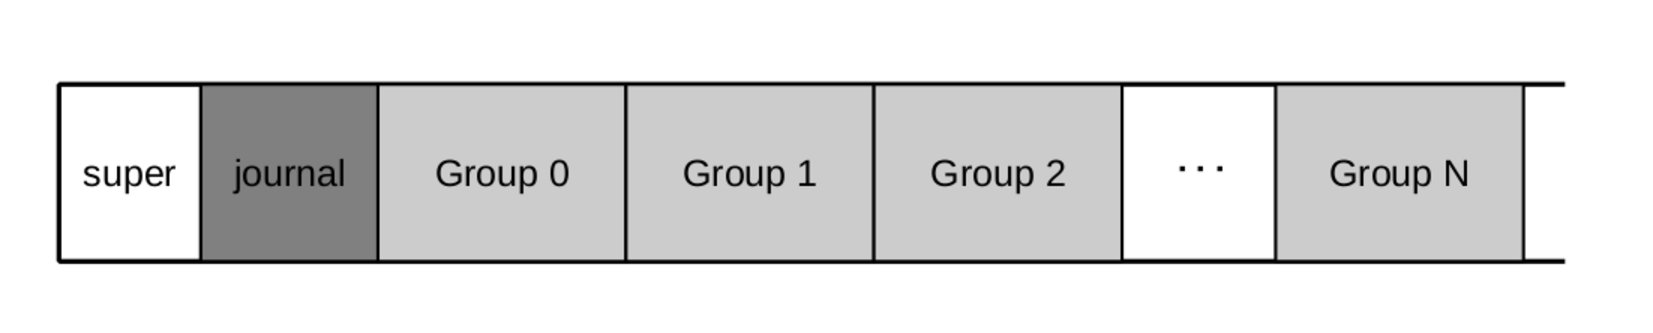
\includegraphics[width=15.0cm,clip]{images/ext3.pdf}
		\caption{ext3 file system の構造}
		\label{fig:ext3}
	\end{center}
\end{figure}
 journaling には, data journaling と metadata journaling が存在する.data journaling は,メタデータと実データの両方を journaling の対象にするものであり,信頼性を重視している.一方で, metadata journaling は,メタデータのみを journaling の対象にするものであり,書き込みの速度を重視している.ここでは, metadata journaling を説明する.\\
 すべてのデータを journaling の対象とすると,それらの書き込みを 2 回ずつ行わなければ行けないため,高いコストが必要になる.そこで,実データは journal に書き込まず,メタデータのみを journaling の対象とした metadata journaling が利用される.これは, ordered journaling とも呼ばれる.\\
 先ほどのクラッシュが起こった際の例で扱った簡単な書き込みを使って, metadata journaling の手順を説明する.最初に,実際に書き込みを行う前に journal に書き込まれるものは,図\ref{fig:metaj}のようになっている.また, TxB は, トランザクションの始まりを意味しており, TxE は,トランザクションの終わりを意味している.
\begin{figure}[H]
	\begin{center}
		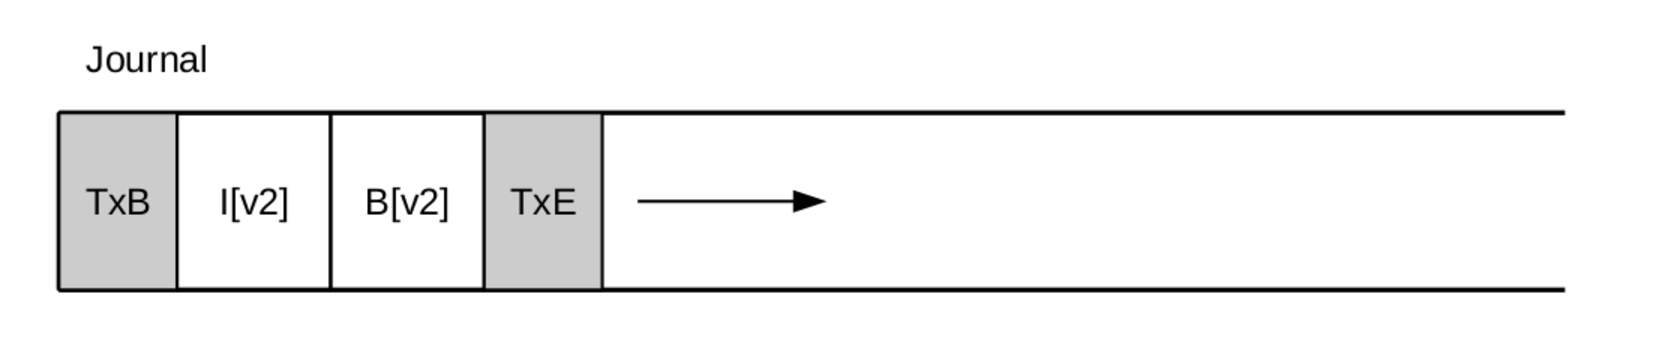
\includegraphics[width=15.0cm,clip]{images/journalLog.pdf}
		\caption{journal log の中身}
		\label{fig:metaj}
	\end{center}
\end{figure}
 書き込み操作によって行われる更新は, inode I[v2], data bitmap B[v2], data block Db の 3 つから構成されている.この内,最初の 2 つがメタデータにあたる.したがって, journal に記録され,記録が無事終わったあとで file system に書き込みが行われる.それに対し,最後の一つは実データである.したがって, file system に一度だけ書き込みが行われるのみである.\\
 ここで,書き込みの順序を考える.例えば,メタデータである inode I[v2] と data bitmap B[v2] の書き込みを行ったあとに, data block Db の書き込みを行うとする.この場合, もし書き込み途中で OS のクラッシュなどが発生して書き込みが中断されてしまうと, file system の一貫性は保たれているが, inode I[v2] は, garbage data を指してしまう状況が生まれる.これは,中断が発生して復帰した時, inode I[v2] と data bitmap B[v2] は書き込みがもう一度行われるのに対し, data block Db は journaling の対象にしていないため,書き込みのやり直しが発生しないからだ.\\
 この状況が発生しないようにするため,多くの場合,実データを書き込んでから,それに関連するメタデータの書き込みを行う.よって,metadata journaling の手順は以下のようになる.\\
\begin{enumerate}
	\item{Data write}\\
	 最終的に実データを書き込む場所に,実データの書き込みを行う.\\
	 書き込みの終了を待つ.
	\item{Journal metadata write}\\
	 TxB block とメタデータを journal log に書き込む.\\
	 書き込みの終了を待つ.
	\item{Journal commit}\\
	 TxE block を journal log に書き込む.\\
	 書き込むの終了を待つ.\\
	 トランザクションがコミットされる.
	\item{Checkpoint metadata}\\
	 最終的にメタデータを書き込み場所に,メタデータの書き込みを行う.\\
	\item{Free}\\
	 journal log のトランザクションを書き込んだスペースを解放する.\\
\end{enumerate}
 さらに, metadata journaling のタイムラインを図\ref{fig:timeline}に示す.各列が,いずれかの要素の write が発行された,あるいは write が完了した論理時間を示している.\\
\begin{figure}
	\begin{center}
		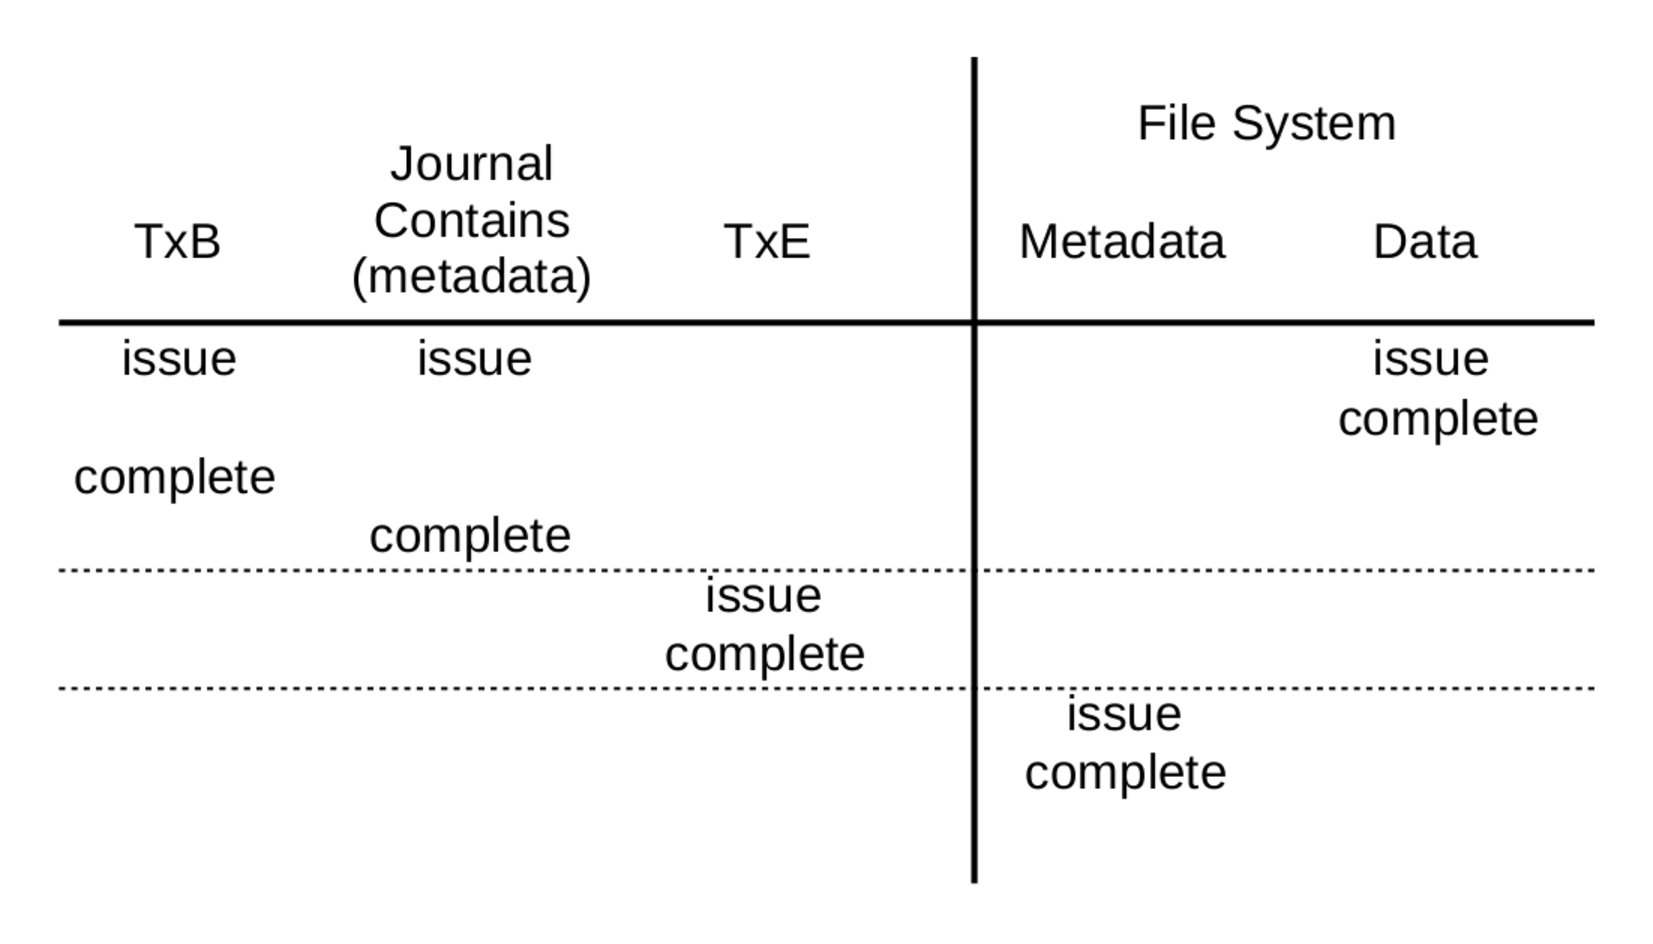
\includegraphics[width=13.0cm,clip]{images/timeline.pdf}
		\caption{metadata journaling timeline}
		\label{fig:timeline}
	\end{center}
\end{figure}
 では, metadata journaling の各手順中にクラッシュなどによって中断され,その後に復帰する場合を考える.\\
\begin{itemize}
	\item{Data write が中断された場合}\\
	復帰後に, journal を見ても何も log が残っていないため,書き込み自体がなかったことになる.したがって, file system の一貫性は保たれた状態である.\\
	\item{Journal metadata write が中断された場合}\\
	復帰後に, journal を見ると途中まで書かれているが,トランザクションの終了を表す TxE が書き込まれていないため,実データはすでに書き込まれているが,書き込み自体はなかったことになる.したがって, file system の一貫性は保たれた状態である.\\
	\item{Journal commit が中断された場合}\\
	この場合, Journal metadata write が中断された場合と同様であるため, file system の一貫性は保たれた状態である.\\
	\item{Checkpoint metadata が中断された場合}\\
	復帰後に, journal を見ると,トランザクションが残っている.そこで,最終的にメタデータを書き込む場所へのメタデータの書き込みを再実行することができる.その結果,書き込みは完了される.したがって, file system の一貫性は保たれた状態である.\\
\end{itemize}
 Linux では,このような journaling 機能を備えた ext4 file system を採用している.さらに LXC は,コンテナ間で file system を共有しているため,複数のコンテナからの I/O リクエストを一つの journal でシリアライズし,順番に処理を行う必要がある.

\clearpage
\section{Linux コンテナに対する DDoS 攻撃}
\label{sec:DDoS}
 第\ref{sec:LXC}章において, LXC が Linux カーネル機能の一つである cgroup を利用して,コンテナ間の isolation を保っていることを説明した.しかし, cgroup による isolation は不完全なものである.本章では,コンテナ上で,あるプロセスを実行することによって,コンテナ間の isolation が保たれなくなることを示す.\\
\subsection{実験環境}
 今回の実験環境とその準備手順について説明する.ホストマシンには,\{-----\}を使用する.使用する OS は, Ubuntu 16.04.1 Server 64bit Linux distribution で,カーネルのバージョンは,Linux 4.4.0-53-generic である. file system には, ext4 file system を使い, journaling mode は,初期設定の状態である, metadata のみ journaling の対象とする ordered journaling とする.正確に性能を記録できるようにするため, LVM を使わないで OS のインストールを行う.コンテナの disk へのアクセスの制限は, cgroup によって行い, Linux コンテナには, LXD 2.0.8 を使用する.\\
 LXD を用いて, ubuntu 16.04.1 のイメージから 2 つコンテナを作成する.このコンテナをそれぞれコンテナ A ,コンテナ B とする.cgroup の blkio サブシステムによって,両コンテナの disk へのアクセスに対して,制限をかける.コンテナ A は 85\% に制限し,コンテナ B は 15\% に制限する.cgroup の制限を有効にするため,スケジューラを Complete Fair Queuing (CFQ) スケジューラに設定する.コンテナ A では,攻撃対象に設定したプログラムを動かし,コンテナ B では,悪意のあるコンテナとして,攻撃プログラムを実行する.\\

\subsection{DDoS 攻撃}
 LXC における cgroup による isolation は不完全なものである.それによって,一つのコンテナから他のコンテナに対して,攻撃ができてしまうことを示す.\\
 disk へのアクセスを 85\% に制限した,攻撃対象のコンテナ A では, Flexible I/O (FIO) benchmark を実行する. FIO benchmark の設定は次のようになっている.workload の種類は sequential write である.キャッシュを使わないように Direct I/O で実行する.\\
 disk へのアクセスを 15\% に制限した,攻撃側のコンテナ B では, FIO benchmark を実行する. FIO benchmark の設定は次のようになっている. workload の種類は sequential write である.キャッシュを使わないように Direct I/O で実行する.100 命令に 1 回 fsync を行う.\\
 結果を図\{-----\}に示す.\\
%\begin{figure}[H]
%\end{figure}
 攻撃対象となる FIO は、 cgroup によって disk へのアクセスを 85\% に制限したため, 85\% のパフォーマンスを示すはずである.しかし,図\{-----\}を見ると, 40\% しか使えていない.したがって,攻撃側のコンテナから攻撃対象となるコンテナに対して,攻撃ができていることがわかる.\\

\clearpage
\section{コンテナにおける資源管理の脆弱性解析}
 第\ref{sec:DDoS}章において, cgroup による isolation が不完全であることを示した.しかし, FIO benchmark が,実際のコンテナで利用されることは少ない.そこで本章では, cgroup による isolation が不完全なことによって,実際のコンテナで使われるものに対しても,他のコンテナから攻撃が出来,攻撃対象のパフォーマンスを下げることができることを示す.
\label{sec:analysis}

\clearpage
\section{関連研究}
\label{sec:relative}

\clearpage
\section{まとめ}
\label{sec:conclusion}

\end{document}